\section*{Chapter 9: Convolutional Networks}
%\section*{Probabilities}
%\subsection*{Expect, Var, Cov, Bay}
%$\E[X]=\int_{\Omega}xf(x)\di x=\int_{\omega}x\Prob[X{=}x]\di x$ \\
\subsection*{Convolutions}
\textbf{Convolution:} $(f*h)(u) = \int_{\mathbb{R}} h(u-t)f(t)dt = \int_{\mathbb{R}} f(u-t)h(t)dt = (h*f)(u)$ 

\textbf{Conv. is shift equivariant:} $f_{\Delta}*h = (f*h)_{\Delta}$

\textbf{Discrete conv.:} $(f*h)[u] = \sum_{t=-\infty}^{\infty}f[t]h[u-t]$

\textbf{Cross-correl.:} $(h\star f)(y) = \int_{\mathbb{R}} h(t)f(y+t)dt$

\textbf{2-D:} $(F*G)[i,j] = \sum_{k=-\infty}^{\infty}\sum_{l=-\infty}^{\infty}F[i-k, i-l] \cdot G[k,l]$

\subsection*{CNNs}
\textbf{Pros}: param sharing, more efficient, translation equivariance, sparse connectivity. \textbf{Cons}: not all data is trans. equiv. and receptive field makes it hard to connect distant features.

\textbf{Padding.} Used to handle borders. \emph{Same padding} pads with zeros and ensures output is of same size (breaks transition equivariance). \emph{Valid padding} only applies conv in the available signal (conv is exact but reduces size). \emph{Other ideas} e.g. reflecting borders to keep transition equivariance.

\textbf{Receptive fields}. CNNs units only have info about close points. By increasing depth, the receptive field increases and can reach further info.

\textbf{Pooling}. Used to locally combine activities by applying a function on each window e.g. max or avg.

\textbf{Strides}. Sub-sampling to reduce size of feature maps. Apply kernel (or pooling) each n pixels. Loss of info.

\textbf{Channels}. Learn multiple filters/kernels per layer. Add dimensions.

\subsection*{CNNS in CV}
Usually use RelU or Leaky ReLU as activation. Vanishing gradients with depth. They have a pyramidal architecture: stack convs reducing resolution while increasing channels.

\textbf{AlexNet}. Pyramidal CNN arch (1.3M+ params) + 3FC (177M+ params)

\textbf{VGG}. Very deep CNN. Only uses convs and it is transition invariant. Uses kernels 3x3 and takes the size down to $1\times N_{classes}$ and apply softmax.

\textbf{Inception}. Uses 1x1 conv to reduce input size by combining info across channels. Concatenates output from diff filter sizes to learn more. Includes sofmax layers at intermediate steps to ease backprop and avoid vanish grads.

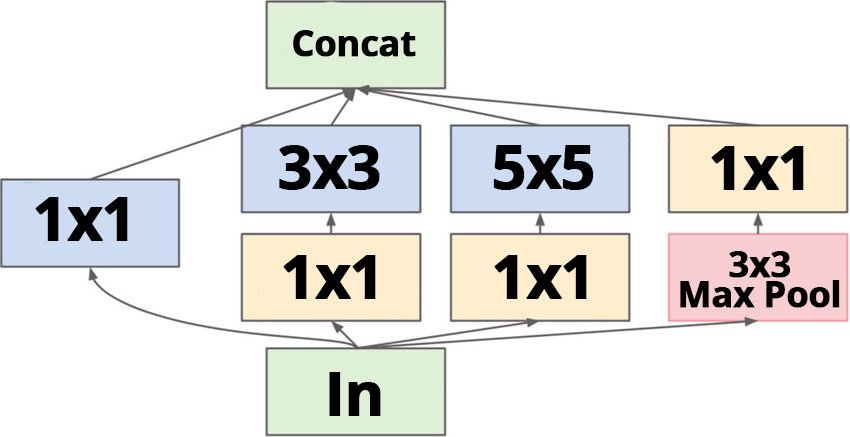
\includegraphics[width=0.6\columnwidth]{src/custom-inception.jpg}

\subsection*{CNNs shapes and parameters}
Given an input $(N, C_{in}, H_{in}, W_{in})$, the output of the conv. is $(N, C_{out}, H_{out}, W_{out})$:

$H_{out} = \lfloor \frac{H_{in}+2 \cdot padding[0] - (kernel\_size[0] - 1)}{stride[0]} + 1 \rfloor $

$W_{out} = \lfloor \frac{W_{in}+2 \cdot padding[1] - (kernel\_size[1] - 1)}{stride[1]} + 1 \rfloor $

The \#params in a layer is: $weights+bias$:

$weights = C_{in} \cdot C_{out} \cdot kernel[0] \cdot kernel[1]$

$bias = C_{out}$

\subsection*{CNNs in NLP}
Map a set of symbols (chars, words, etc.) to a vector space (embedding). Then, apply CNN to the embedding space.

\textbf{Word2Vec}. Uses a log-bilinear model to predict prob. of word $\nu$ appearing in neighborhood of $w$. $p(\nu|w) = \frac{exp[x_w\cdot y_\nu]}{\sum_\mu exp[x_w\cdot y_\mu]}$. Requires summing over vocabulary $\mu$ (expensive). Can use negative sampling to avoid the sum. In this case we only predict prob of appearing together $p(1|\nu, w)$